%-------------------------------------------------------------------------
\section{Method}
Precomputed Radiance Transfer  is a physically-based rendering method to accelerate on-line computations of the (simplified) rendering equation:
\begin{align}
L(\bm{\omega}_0 ) &= 
\int_{\Omega}   L_{\epsilon}(\bm{\omega}_i ) 
\underbrace{f(\bm{\omega}_i,\bm{\omega}_0) 
V(\bm{\omega}_i) H_N(\omega_i) }_{T(\bm{\omega}_i,\bm{\omega}_0) }
\,  \, d\bm{\omega}_i 
\label{rendering equation PRT}
\end{align}
where $L_{\epsilon}$ accounts for all incoming radiance over the hemisphere, $f$  describes the surface reflectance properties $f$ (BRDF), $H_N$ is the Lambert's Law and $V$ the visibility function describing geometric information of the scene. PRT precisely exploits the essence of static/non-deformable objects by uniquely determining the integrand $T(\bm{\omega}_i,\bm{\omega}_0)$ (called the \textbf{transfer function}), which contains the costly-to-compute  visibility term,
\begin{align*}
V :  \mathcal{S}  \times \Omega \rightarrow \{0,1\} \quad
\end{align*}
for each surface point $\bm{s} \in \mathcal{S} \subset \mathbb{R}^3$ \cite{CohenBook}. 

Both functions $L_{\epsilon} $ and $T$  are projected onto a suitable set of orthonormal basis functions for faster evaluation of the rendering equation \ref{rendering equation PRT}. 
For $m$ number of coefficients of the basis functions and $l_i$, $t_i$ being the $i$-th coefficient of $L_{\epsilon} $ and $T$ respectively, equation \ref{rendering equation PRT} reduces to, \cite{sloan2002precomputed} 
\begin{align}
L(\bm{\omega}_0 ) \approx \sum_{j}^{m} l_j \cdot t_j 
\label{Eq: Reduced Rendering Eq}
\end{align}
We chose a \textit{Spherical Harmonics} (SH) basis to encode the transfer function $T$ and the light environment $L_{\epsilon}$.

As mentioned above, our aim is to extend the PRT method to malleable and dynamic objects, but avoiding costly precomputations and storage of every single transfer function $T_i$ per shape query $S_i$ (with $i \in [1,2,\dots, d]$ and $d$ : $\#$ deformations ).

With this in mind, we suggest a data-based model, a fully convolutional neural network, to infer the transfer function $T_i$ for any given shape query $S_i$. 
This makes the costly ray-casting computations superfluous and solves the exorbitant memory requirements, only necessitating the storage of the network's parameters.

Moreover, by choosing to estimate the transfer function, instead of a direct prediction of $L$, our method is flexible to dynamic light environments (see figure \ref{Fig: Varying lighting}).
%------------------
% FIGURE (Varying Lighting)
\begin{figure}[H]
  \centering
    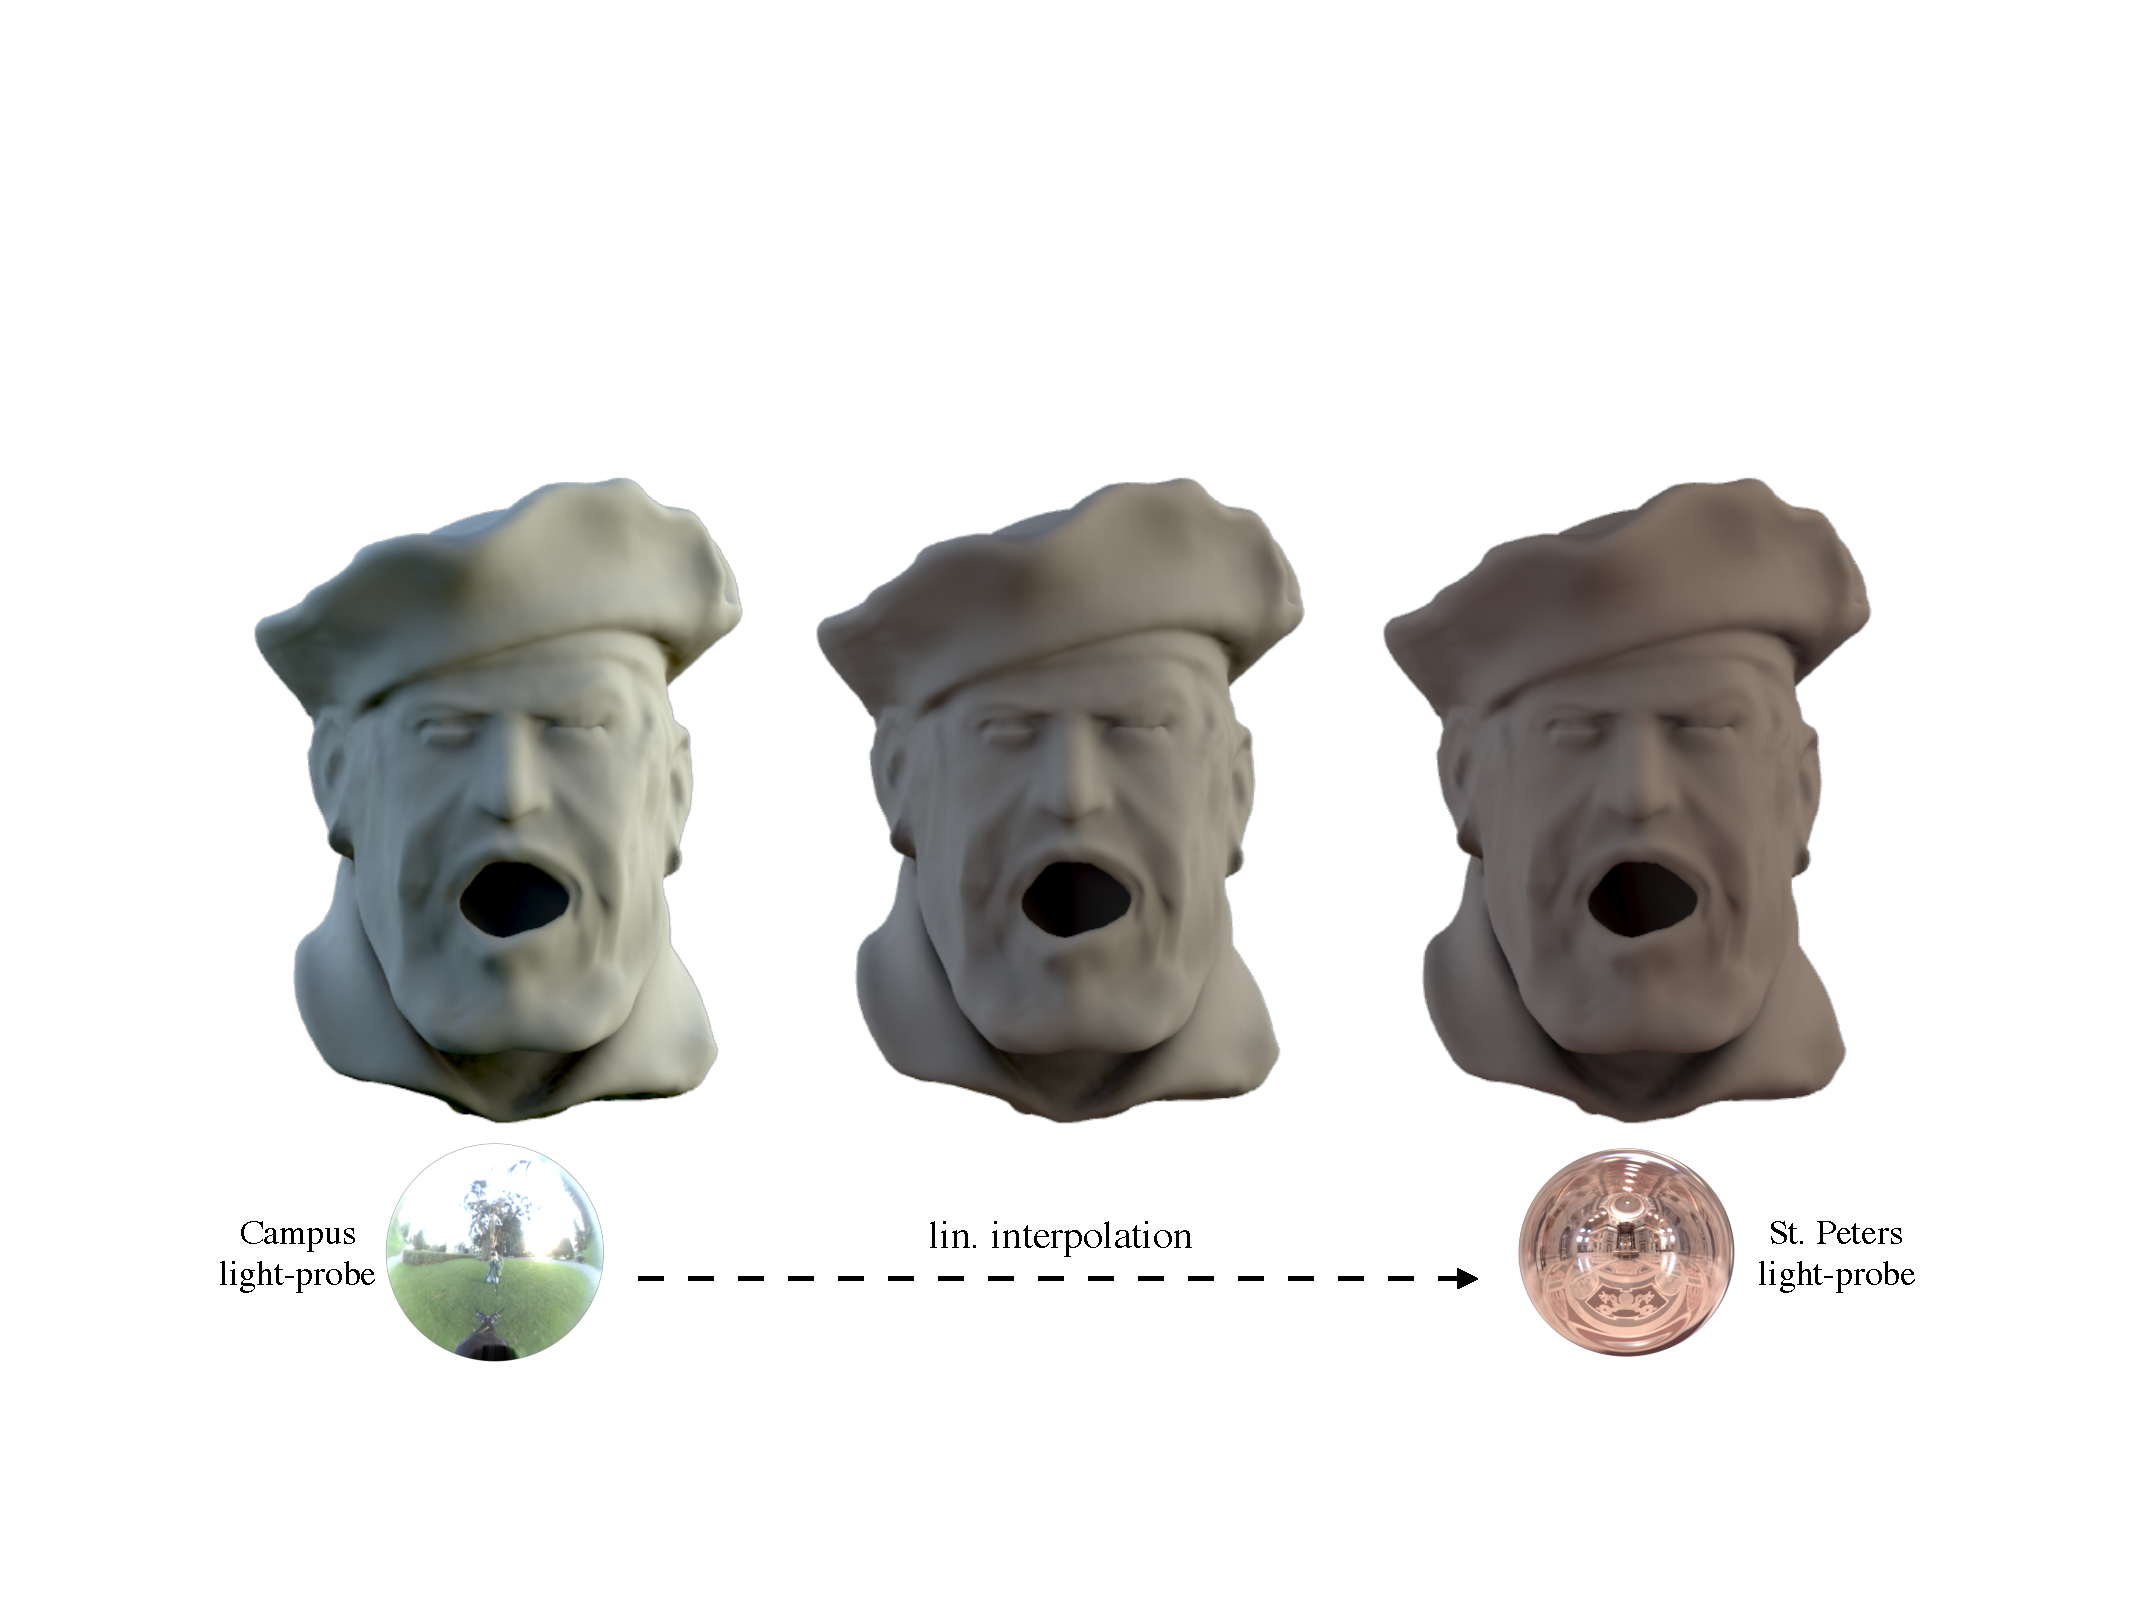
\includegraphics[width=1.0\textwidth]{Figures/varying_lighting}
     \caption{Dynamic lighting. Rendered appearance of the \textit{Pirate Head} under three different  lighting conditions. Lighting is interpolated between two light-probes.}
     \label{Fig: Varying lighting}
\end{figure}
%------------------
%%%%%%%%%%%%%%%%%%%%%%%%%%%%%%%%%%
% -------------- GEOMETRY IMAGE ----------------- 
%%%%%%%%%%%%%%%%%%%%%%%%%%%%%%%%%%
\subsection{Data: Geometry Images}
We propose learning directly \textbf{on} the object's surface in order to leverage its underlying shape structure and further to be consistent with regular animated surface geometry representation for real-time rasterization. Geometry images present a planar and regular shape representation on which standard 2D CNNs can be applied \cite{gu2002geometry, sinha2016deep}. Surfaces with a single boundary (topological disks) are mapped onto a unit square and later discretized (or re-sampled) into a regular grid of $n \times n$ vertices. We chose harmonic map (HM) as implicit parametrization of the interior of the 2D domain \cite{HM_book, HarmonicMapping}. Further, our intent is that, for practically zero genus object surfaces, HMs provide the conditions for a homomorphism with diffeomorphic interior mapping such that the mapped differentiable manifold takes place smoothly in the image domain.
%In a \textit{Stretch-Minimising} parametrisation is presented for the interior of the planar surface. However, for simplicity, but without loss of generality, ...

Importantly, we apply deformations only on the reconstructed object (shape $\mathcal{S_R}$ in Figure (1) ) in order to make our shape representation, geometry images, invariant to deformations. By doing so, we maintain a one-to-one pixel correspondence between deformations; hence, filtering out deformation invariant information of the representation; and therefore, facilitating the feature extraction of surface properties that are more closely related to self-shadowing and light transfer effects. Moreover, this also means that the conversion process of a surface into a geometry image is required only once and can be performed off-line, saving precious computation time.

In addition to position values  $\mathcal{P}$, we use surface normals $\mathcal{N}$ as regressor for the network, where 
\begin{align*}
	\mathcal{P} = [ P_x, P_y, P_z ]^T , \quad
	\mathcal{N} = [ N_x, N_y, N_z ] ^T 
\end{align*}
and  $P_i, N_i \in \mathbb{R}^{n \times n }$ being each coordinate image  $i \in \{ x,y,z\}$ of positions and normals respectively. 

In result, our network predicts a corresponding sequence of images $\mathcal{T_{D,G}}$,
\begin{align*}
	f_{CNN} (  \mathcal{P} , \mathcal{N} ) = 
	\begin{cases}
	\mathcal{T_D}  & \text{diffuse} \\
	\mathcal{T_G} & \text{glossy}
	\end{cases}
\end{align*}
which, for \textbf{diffuse materials}, consists of the SH-coefficients of the transfer function of the input shape, as introduced above (see equation \ref{Eq: Reduced Rendering Eq}):
\begin{align*}
	\mathcal{T_D} = [ t_1, t_2, \dots, t_m ]^T \in \mathbb{R}^{m \times n \times n} 
\end{align*}
that is, pixel $i$ of image $t_j$ represents the transfer coefficient $j$ of vertex $i$ of the input surface.

For \textbf{glossy materials}, our network predicts the transferred radiance $\mathcal{T_G}$ consisting of three radiance channels, 
\begin{align*}
\mathcal{T_G} = [R_r , R_g ,R_b]^T \in \mathbb{R}^{3 \times m \times n \times n} 
\end{align*}
resulting from the product between the transfer matrix $M_T$ and the lighting coefficients  $ L^{sh}_i$ \cite{sloan2002precomputed}. 
\begin{align*}
R_i= M_T \cdot L^{sh}_i   \in \mathbb{R}^{m \times n \times n}   \quad \text{for }~  i \in \{r,g,b\} .
\end{align*}

%%%%%%%%%%%%%%%%%%%%%%%%%%%%%%%%%%
% -------------- NETWORK ----------------- 
%%%%%%%%%%%%%%%%%%%%%%%%%%%%%%%%%%
\subsection{Network and Performance }
\subsubsection*{Architecture: \\} 
Our deep convolutional network is configured as a \textit{U-Net}  \cite{U-Net}, consisting of an \textit{encoder} and \textit{decoder} with \textit{skip-connections}. Both encoder and decoder consist of sequences of \textit{ResNet} blocks \cite{ResNet} each comprising a series of \textit{2D-convolutions}, \textit{batch-normalisation} and \textit{ReLU} activation layers (illustrated in Figure (\ref{Fig: NetworkTopology}) ). For the last layer of the decoder we use a \textit{sigmoid} activation function. Instead of a \textit{pooling-layer} we perform down-sampling by increasing the stride, by a factor of two, within a convolutional layer \cite{StridingConv}. To avoid information loss,  we make use of skip-connections passing information between outputs of encoding layers and corresponding inputs of the decoding layers.

\subsubsection*{Synthesis of Training Data:\\}
We generate the training data applying sequences of free form deformations onto a given object. Specifically, for our experiments, deformations are generated either by a physically driven simulation or by linear combinations of blendshapes (figure \ref{Fig: DPRT_Quality}). We also refer readers to the supplementary video. 

Each generated deformation sequence has a total length of 500 frames. 
At each frame $i \in [1,2,\dots,500]$ we store the position $\mathcal{P}_i$  and normal $\mathcal{N}_i$ images of the current deformation, and perform a full integration using ray samples to compute the corresponding ground truth $\mathcal{T_D}_i$ or $\mathcal{T_G}_i$. For our experiments we chose a SH-band number of $4$, which corresponds to $16$ coefficients. Moreover, we experimented with image resolutions of $256 \times 256$ and $512 \times 512$. 

Our implementation for the generation of the ground truth data $\mathcal{T_{D,G}}$ requires a duration of $39.6$s for diffuse and $49.7$s for glossy surfaces, per frame.

\subsubsection*{Training: \\} 
The data is split into a training and validation set consisting of $450$ and $50$ data samples respectively. As cost function, we minimize the pixel-wise absolute error between predicted output and the ground-truth ($L_1$-loss), and the optimizer we use is ADAM \cite{ADAM}. 

Convergence varies from object to object, but in most cases $500$ to $1000$ epochs are sufficient, whereby we used a batch size of 5. The network is implemented in Keras with Tensorflow as backend \cite{Keras} and takes close to $16$ hours to compute $800$ epochs of training on a single NVIDIA GetForce GTX 2080 GPU.

\subsubsection*{Runtime: \\}
\label{sec:runtime}
In order for \textit{DeepPRT} to function in real-time, fast network inference is required. However, to achieve good approximations existing deep neural networks, such as ours, rely on very deep architectures with sufficient quantities of parameters. 
In particular, our network has approximately $11.8$ million parameters, occupying $45$Mbytes of CPU memory, and with an inference time of $45$ms on a high-end GPU \textit{NVIDIA RTX 2080}.
In addition, for a network input size of $4.5$Mbytes there is a further upload (loading input images, $\mathcal{P}$ and $\mathcal{N}$, from CPU into the GPU) cost of approximately $5$ms.  

After prediction, the performance for the rendering process differs notably between diffuse and glossy surfaces: 
For \textbf{diffuse} surfaces, the dot product between predicted transfer coefficients $\mathcal{T_D}$ and the three channels of the lighting coefficients are calculated (eq. \ref{Eq: Reduced Rendering Eq}) and the result passed to the buffers for final rendering.  For our sample geometries with $256^2$ number of vertices the computation of the dot product takes $13$ms on the GPU, and an upload time of $0.09$s for the resulting $4.0$Mbytes exiting radiance vectors.
On the other hand, the output of the network for \textbf{glossy} surfaces $\mathcal{T_G}$ is three times the size as for diffuse objects, thus for the same sample geometry as above, it occupies $12.0$Mbytes. For further rendering,  $\mathcal{T_G}$ is convolved with a BRDF-kernel, based on Kautz et al. \shortcite{ BRDF_kernel}, before passed to the shaders \cite{sloan2002precomputed}.  We perform these steps in the CPU resulting in an additional duration of $1.29$s. 

We note that our implementation is far from being optimal.  Both, the rendering and the prediction process can be accelerated significantly. It has been extensively shown that most neural network models are highly compressible and can be significantly accelerated, eventually making them deployable to devices with low memory resources and applicable in real-time \cite{Deep_Compression, Survey_NN_Compression}.
Nevertheless, exploring network optimization methods reaches beyond the scope of this work. Hence, for our experiments we used the uncompressed U-Net introduced above. In section \ref{Sec: memory_savings} we show that even neglecting network optimization our DeepPRT approach already achieves immense memory savings, compared to traditional PRT. 
%%%%
\begin{figure*}[t]
  \centering
    \includegraphics[width=1.0\textwidth]{Figures/Network_topology.pdf}
     \caption{\textit{Left:} Illustration of the configuration of our U-shaped network. \textit{Right:} Shows the two kind of operations performed within our ResNet blocks.}
     \label{Fig: NetworkTopology}
\end{figure*}

  


